\chapter{Analisi dei Requisiti}
\section{Descrizione dei requisiti in linguaggio naturale}
\label{sec:req}
La descrizione che segue riporta, in linguaggio naturale, una sistesi dei requisiti necessari per la creazione del sistema informativo:
\mline
\textit{
  Si desidera realizzare un sistema informatico per archiviare le informazioni riguardanti i dati astrologici di più individui.
  L'astrologia non è altro che un complesso di credenze secondo cui le posizioni e i movimenti dei corpi celesti rispetto alla Terra influiscono sugli eventi umani collettivi e individuali. È infatti usata per il riscontro di caratteristiche comportamentali delle persone, in base alla loro data, ora e luogo di nascita.%\newline
  Si vuole pertanto memorizzare la situazione celeste al momento della nascita degli individui, la quale prende il nome di Tema Natale, o Carta Natale.\\
  I Segni Zodiacali dell'astrologia comune sono 12, ed ognuno ha un suo numero. I segni sono infatti numerati, partendo dal primo che è l'Ariete si termina coi Pesci per poi ripartire, creando un ciclo senza fine. Ogni segno possiede un nome, ed è definito da un Modo e da un Elemento. Questi ultimi sono rispettivamente solo 3 e 4, ed anche essi si ripetono ciclicamente per ogni segno (Il primo segno avrà il primo modo e il primo elemento, il quarto segno avrà il primo modo e il quarto elemento e così via).\\
  Le Case Astrologiche sono anch'esse 12, ognuna ha un numero che definisce l'ordine in senso antiorario rispetto all'est, e un nome.
  Ogni casa ha un segno zodiacale che la governa, indipendentemente dalla persona, che coincide sempre con il segno che ha lo stesso numero della casa.\\
  Ogni Pianeta può trovarsi sotto un determinato segno in una determinata casa, dipendentemente dall'individuo. Allo stesso modo si comportano altri "punti", per esempio, un nodo lunare viene trattato come un pianeta, anche se non esiste un corpo fisico nello spazio che lo rappresenta. Gli estremi del cielo e dell'orizzonte sono 4 e cadono sempre sulle stesse case, ma i segni dipende dalla persona presa in considerazione.\\
  Alcuni pianeti e altri punti simbolici possono essere Retrogradi al momento della nascita (in breve, sembra che girino al contrario rispetto a come dovrebbero), si desidera memorizzare anche quest'informazione se presente.
  Ogni pianeta ha dei segni zodiacali affini, fino a due. Quando un pianeta si trova sotto un segno affine, si dice che è in Domicilio.\\
  Gli Aspetti sono angoli creati tra due pianeti/punti. Gli aspetti più importanti sono 5, ma ce ne sono altri meno conosciuti. Ognuno è definito da un Grado specifico e da un Nome. Una persona può avere più aspetti che legano un signolo pianeta/punto ad altri, ma un pianeta/punto può anche non avere aspetti.\\
  Per ogni persona è necessario memorizzare Nome, Cognome, Data di Nacita, Ora di Nascita e Luogo di Nascita.
  Non è importante memorizzare necessariamente tutte le informazioni possibili. Se si vuole per esempio memorizzare il solo segno solare di qualcuno, deve essere possibile farlo.
  Si vuole permettere l'aggiunta e la rimozione di Persone dal sistema.\\
  Si vuole permettere l'aggiunta, la rimozione e la modifica di informazioni astrologiche per le persone presenti nel sistema.\\
  Inoltre, si vorrebbe aggiungere qualche funzione in grado di contare per esempio il numero di segni di uno specifico elemento posseduti da una persona, e simili.
}
\mline
\section{Estrazione dei concetti principali}
Il problema posto non è affatto semplice da spiegare a parole, ma è possibile capire meglio i concetti chiave evidenziando le parole più importanti.
\mline
\textit{
  [...] I \textbf{Segni Zodiacali} dell'astrologia comune sono 12, ed ognuno ha un suo numero. I segni sono infatti numerati, partendo dal primo che è l'Ariete si termina coi Pesci per poi ripartire, creando un ciclo senza fine. Ogni segno possiede un nome, ed è definito da un \textbf{Modo} e da un \textbf{Elemento}. Questi ultimi sono rispettivamente solo 3 e 4, ed anche essi si ripetono ciclicamente per ogni segno (Il primo segno avrà il primo modo e il primo elemento, il quarto segno avrà il primo modo e il quarto elemento e così via).\\
  Le \textbf{Case Astrologiche} sono anch'esse 12, ognuna ha un numero che definisce l'ordine in senso antiorario rispetto all'est, e un nome.
  Ogni casa ha un segno zodiacale che \textbf{la governa}, indipendentemente dalla persona, che coincide sempre con il segno che ha lo stesso numero della casa.\\
  Ogni \textbf{Pianeta} può trovarsi sotto un determinato segno in una determinata casa, dipendentemente dall'individuo.\\
  Allo stesso modo si comportano altri \textbf{"punti"}, per esempio, un nodo lunare viene trattato come un pianeta, anche se non esiste un corpo fisico nello spazio che lo rappresenta. Gli \textbf{estremi del cielo e dell'orizzonte} sono 4 e cadono sempre sulle stesse case, ma i segni dipende dalla persona presa in considerazione.\\
  Alcuni pianeti e altri punti simbolici possono essere \textbf{Retrogradi} al momento della nascita (in breve, sembra che girino al contrario rispetto a come dovrebbero), si desidera memorizzare anche quest'informazione se presente.\\
  Ogni pianeta ha dei segni zodiacali affini, fino a due. Quando un pianeta si trova sotto un segno affine, si dice che è in \textbf{Domicilio}.\\
  Gli \textbf{Aspetti} sono angoli creati tra due pianeti/punti. Gli aspetti più importanti sono 5, ma ce ne sono altri meno conosciuti. Ognuno è definito da un Grado specifico e da un Nome. Una persona può avere più aspetti che legano un signolo pianeta/punto ad altri, ma un pianeta/punto può anche non avere aspetti.\\
  Per ogni \textbf{persona} è necessario memorizzare Nome, Cognome, Data di Nacita, Ora di Nascita e Luogo di Nascita.
  [...]
}
\mline
È importante capire fin da subito quali sono precisamente le specifiche, pertanto, a seguire, verranno spiegate più dettagliatamente alcune parti del testo per approfondire meglio i concetti.
\mline
\textit{
  I \textbf{Segni Zodiacali} dell'astrologia comune sono 12, ed ognuno ha un suo numero. I segni sono infatti numerati, partendo dal primo che è l'Ariete si termina coi Pesci per poi ripartire, creando un ciclo senza fine. Ogni segno possiede un nome, ed è definito da un \textbf{Modo} e da un \textbf{Elemento}. Questi ultimi sono rispettivamente solo 3 e 4, ed anche essi si ripetono ciclicamente per ogni segno (Il primo segno avrà il primo modo e il primo elemento, il quarto segno avrà il primo modo e il quarto elemento e così via).
}
\mline
Dovrebbe risultare chiaro che esiste un numero finito di segni zodiacali. Quel che potrebbe non risultare chiaro è il funzionamento dei Modi e degli Elementi. Possiamo vedere  i Segni, i Modi, e gli Elementi come liste circolari di elementi finiti. Esistono solo tre Modi (Cardinale, Fisso, Mutevole) e quattro elementi (Fuoco, Terra, Aria, Acqua) ordinati come qui riportati.\newline
Il primo Segno, Ariete, sarà del tipo del primo modo (Cardinale), e il suo elemento sarà il primo (Fuoco).\newline
Il secondo Segno invece, Toro, sarà del tipo del secondo modo (Fisso), e il suo elemento sarà il secondo (Terra).\newline
Una volta arrivati al quarto segno i modi a disposizione saranno terminati, e sarà necessario ricominciare dal primo. Il Cancro sarà quindi del tipo del primo Modo (Cardinale), e il suo elemento sarà il quarto (Acqua).\newline
Il Segno successivo, Leone, sarà del tipo del secondo modo (Fisso), e dato che sono finiti gli elementi, si ricomincia da capo. L'elemento del Leone sarà il Fuoco.\newline
E così via fino al dodicesimo segno.\newline
Usando matematica di base quindi, notiamo che esistono tre segni per ogni elemento, e quattro per ogni modo.
\mline
\textit{
  Le \textbf{Case Astrologiche} sono anch'esse 12, ognuna ha un numero che definisce l'ordine in senso antiorario rispetto all'est, e un nome.
  Ogni casa ha un segno zodiacale che \textbf{la governa}, indipendentemente dalla persona, che coincide sempre con il segno che ha lo stesso numero della casa.
}
\mline
Esistono quindi anche un numero finito di Case, proprio come i segni esse sono 12, ed esiste una corrispondenza 1:1 tra i due che vale sempre.
\mline
\textit{
  Ogni \textbf{Pianeta} può trovarsi sotto un determinato segno in una determinata casa, dipendentemente dall'individuo.\\
  Allo stesso modo si comportano altri \textbf{"punti"}, per esempio, un nodo lunare viene trattato come un pianeta, anche se non esiste un corpo fisico nello spazio che lo rappresenta. Gli \textbf{estremi del cielo e dell'orizzonte} sono 4 e cadono sempre sulle stesse case, ma i segni dipende dalla persona presa in considerazione.
}
\mline
I pianeti sono quindi da intendersi come corpi fisici presenti nello spazio. Si ricorda che in astrologia, il Sole, la Luna e Plutone sono considerati Pianeti per semplicità. Gli altri pianeti più importanti sono gli stessi che troviamo nel sistema solare.\newline
Nel testo, per "punti" sono definiti quelli che non sono a tutti gli effetti classificati come pianeti, ma hanno comunque un ruolo rilevante nel Tema astrologico. Essi si comportano però a tutti gli effetti come pianeti, hanno orbite proprie e cadono sotto case e segni. Nel testo vi è un esempio di un punto astratto, ma in questa categoria possono cadere anche corpi come Chirone, che è classificato come Asteroide.\newline
Possiamo trattare gli estremi allo stesso modo, in quanto anche essi cadono sotto un segno ed una casa, anche se, la casa in questione, é "statica" e non varia mai da persona a persona (per esempio, l'Ascendente cade sempre in prima casa).
\mline
\textit{
  Alcuni pianeti e altri punti simbolici possono essere \textbf{Retrogradi} al momento della nascita (in breve, sembra che girino al contrario rispetto a come dovrebbero), si desidera memorizzare anche quest'informazione se presente.
}
\mline
Scopriamo che un determinato pianeta puo' essere retrogrado, ma cosa vuol dire esattamente?\newline
Immaginiamo di essere alla guida di un'auto. Davanti a noi, sul bordo della strada, vediamo un cavallo che galoppa.
Il cavallo sta procedendo in avanti, ma a un certo punto lo sorpassiamo. Per un paio di secondi osserviamo che il cavallo si muove all'indietro rispetto allo scenario. Questa appena descritta non è altro che un illusione ottica, ma la stessa situazione si verifica nel nostro sistema solare. O almeno, questo è quello che vediamo dalla terra. Nessun pianeta deciderà mai di cambiare orbita casualmente.\newline In questo modo abbiamo ottenuto qualche informazione preziosa. Il sole non potrà mai essere retrogrado dalla prospettiva terrestre, in quanto vi giriamo intorno, e lo stesso vale per la Luna, la quale gira proprio attorno alla terra.\newline
Questo concetto, è estendibile anche ai corpi che non sono pianeti, in quanto, il punto chiave, sta nell'effetto ottico causato dalle orbite. Esistono addirittura punti che sono sempre retrogradi, come nel caso dei due Nodi Lunari.
\newpage
\mline
\textit{
  Ogni pianeta ha dei segni zodiacali affini, fino a due. Quando un pianeta di trova sotto un segno affine, si dice che è in \textbf{Domicilio}.
}
\mline
Domicilio, significa che un determinato Pianeta si trova sotto un segno zodiacale affine, ovvero che lo potenzia in qualche modo. Il sole ha il suo Domicilio solo in Leone, la Luna ha il suo solo in Cancro. Tutti gli altri pianeti, hanno il loro domicilio anche su più di un segno, per esempio, Venere ha Domicilio su Toro e su Bilancia.\newline
Il Domicilio è un concetto affibiato solo ed esclusivamente ai pianeti del sistema solare, più il Sole e la Luna.
\mline
\textit{
  Gli \textbf{Aspetti} sono angoli creati tra due pianeti/punti. Gli aspetti più importanti sono 5, ma ce ne sono altri meno conosciuti. Ognuno è definito da un Grado specifico e da un Nome. Una persona può avere più aspetti che legano un signolo pianeta/punto ad altri, ma un pianeta/punto può anche non avere aspetti.
}
\mline
È importante notare che nel testo, con Aspetto si intende la sola Angolazione tra due punti distinti. Prendiamo l'aspetto "opposizione" per esempio. Con opposizione intendiamo un angolo di 180 gradi tra due punti. Una specifica persona puo' possedere più di un'opposizione nel suo tema Natale (la famosa cantante Taylor Swift ne ha più di 10!), così come può non averne nessuna.\newline
\textbf{Importante}, notiamo una congruenza del tipo:\newline

\begin{align}
  "(Punto A, Aspetto K, Punto B)" \equiv "(Punto B, Aspetto K, Punto A)"
\end{align}
\newpage
\section{Ambiguità}

Chiarifichiamo alcuni termini usati nella Sezione \ref{sec:req} e nel Capitolo \ref{cap:int}:\newline
Il termine \textbf{Aspetto} ha un duplice significato. Si intende per Aspetto l'angolo in gradi tra due pianeti, ma anche le triplette del tipo (Punto1, Angolo, Punto2) riguardati una persona.\newline
Non esistono termini aggiuntivi per separare i due concetti, per cui, in questo documento e sul sistema informatico sarà necessario capire cosa si intende con "Aspetto" in base alla situazione.\newline
Con il termine \textbf{Tabella} che apparirà anche sullo schema concettuale finale che seguirà in Figura \ref{fig:finalscheme} non si intende la tabella fisica del Database finale, ma qualcosa di più semplice. Con tabella intendiamo un riquadro in cui sono mostrati i nostri dati. Catalogare i dati come appaiono in Figura \ref{fig:natal} sarebbe impossibile. Per questo, con \textbf{"Tabella Dei Placement"} si intenderà qualcosa del tipo:

\begin{figure}[H]
\centering
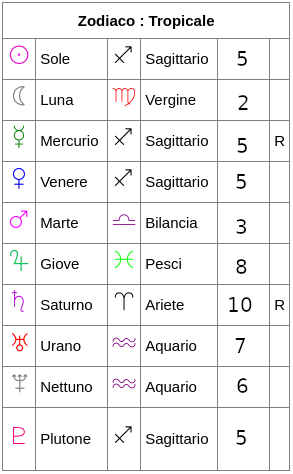
\includegraphics[width=0.4\textwidth,height=0.4\textheight,keepaspectratio]{img/exampleTable.png}
\caption{Tabella dei Placement d'esempio}
\label{fig:exampleTable}
\end{figure}
